\subsection{Widgets}
All the UI in flutter is made by a tree of Widgets. 

Almost all widgets are StatelessWidgets or StatefulWidgets.

\begin{itemize}
    \item immutable;
    \item constructor calls the \texttt{build()} method, that returns the widget;
    \item \texttt{build()} cannot be called again;
    \item new instance must be created in order to redraw the widget;
\end{itemize}

Widgets receive a \texttt{BuildContext} in the \texttt{build()} method .
It is a reference to the location of a Widget in the UI tree and it can contain 
properties concerning the widgets rendering.

\subsection{StatefulWidgets}


\begin{itemize}
    \item Have an associated state object;
    \item State object is mutable and redraws the immutable widget through the \texttt{build()} method;
    \item The \texttt{StatefulWidget} derived class should override at least the 
    \texttt{createState()} method, that returns the associated state object ;
    \item The associated \texttt{State} class should override the \texttt{build()}
    method that returns the \texttt{Widget} (created the first time or redrawn).
\end{itemize}

\begin{lstlisting}
class MyWidget extends StatefulWidget { 
    @override 
    _MyWidgetState createState() => _MyWidgetState(); 
    } 
    
    class _MyWidgetState extends State<MyWidget> { 
    sometype value = initvalue; 
        
    @override Widget build(BuildContext context) { 
        return Container( ...
        // the UI of this widget 
        ); 
    }
}
\end{lstlisting}

\subsubsection{Stateful lifecycle}

\begin{figure}[h]
\centering
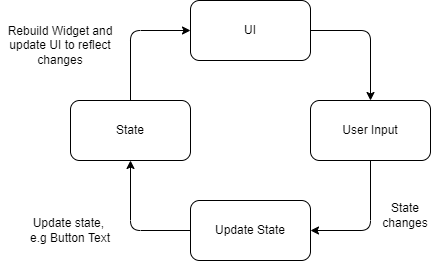
\includegraphics[width=0.8\linewidth]{figures/09_stateful_widget_lifecycle.png}
\caption{Stateful Widget lifecycle}
\label{fig:stateful_widget_lifecycle}
\end{figure}

\begin{itemize}
    \item \texttt{createState()}: Is immediately called after construction;
    \item \texttt{initState()}: Called after creation if overridden; 
    \item \texttt{build()}: To create or redraw a widget tree dependent on the state
    Automatically called if state changes (using \texttt{setState()} or \texttt{didUpdateWidget()});
    \item \texttt{setState()}: Should be called with a function parameter that 
    changes the state and makes a rebuild. 
\end{itemize}

\begin{figure}[h]
\centering
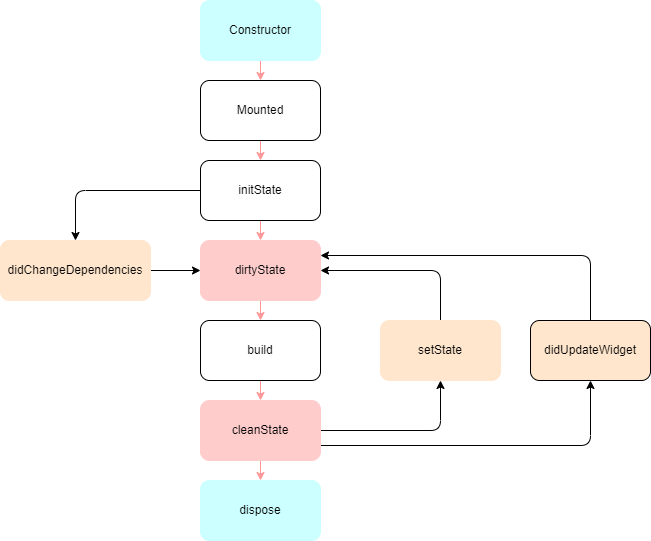
\includegraphics[width=0.8\linewidth]{figures/09_state_object_lifecycle.png}
\caption{State object lifecycle}
\label{fig:state_object_lifecycle}
\end{figure}

\begin{tcolorbox}[colback=red!5,colframe=red!75!black, title=Advantages of stateful widgets over android API]
Supposing that you want to "show a collection of items to a user", or show a list that might be updated, 
in android API, you would have to use an \texttt{ArrayAdapter} or \texttt{BaseAdapter}.  
As explained in the \textbf{Basic Android} chapter, if we want to draw a specific view of the list, we must 
override the ArrayAdapter and create our own view.  

In Flutter, this task is simplified, by using the \texttt{StatefulWidgets}, the collection/list of elements 
is treated as another normal Widget. Everytime the information inside the Widget is updated, it's redrawed 
once again. No overrides are necessary and the code is simplified. 
\end{tcolorbox}




